\documentclass[11pt,a4paper]{article}
\usepackage[margin=2.4cm]{geometry}
\usepackage{amsmath,amssymb,booktabs,graphicx,longtable}
\usepackage{xcolor}
\usepackage[colorlinks=true,linkcolor=blue!45!black,citecolor=blue!45!black,urlcolor=blue!45!black]{hyperref}
\usepackage{titlesec}
\titleformat{\section}{\large\bfseries}{\thesection}{0.6em}{}
\setlength{\parskip}{0.35em}
\newcommand{\pip}{\mathrm{PIP}}
\title{\bf Fine-mapping under a sparse genetic architecture\\[2pt]
\large Iteration 004 benchmark --- complete analysis of the sparse arm}
\author{fmbenchmark}
\date{\today}
\begin{document}\maketitle

\begin{abstract}
\noindent
This report analyses the \emph{sparse} arm of the Iteration 004 fine-mapping
benchmark: 9 design rows, 11{,}250 method fits per method, 18 methods, all
fitted with in-sample LD. It covers overall accuracy, the conditions under
which each method performs well, false-discovery and calibration behaviour,
credible-set economics, and the three ``senses'' of variable importance
(variance-explaining, decision-relevant, diagnostic). Every quantity derived
from posterior inclusion probabilities is defined explicitly in
\S\ref{sec:methods} before it is used, including the estimator's tie handling,
its aggregation level, and the noise correction applied to the variance
decomposition. The headline results are: (i) the number of causal variants $S$
dominates the variance budget everywhere; (ii) the \emph{presence} of
annotations matters and their \emph{strength} barely does; (iii) the
Functional BEATRICE ablation is monotone and significant, with region sharing
contributing more than annotations alone under continuous annotations; and
(iv) the BEATRICE family buys ranking accuracy at a measurable cost in
calibration.
\end{abstract}

\tableofcontents
\bigskip

\section{What was simulated, and what a ``cell'' is}\label{sec:design}

The sparse arm holds the genetic architecture fixed at a \emph{sparse} model:
each region contains exactly $S$ causal variants and no infinitesimal
background. Nine design rows cross the annotation condition with the
enrichment level:

\begin{center}\small
\begin{tabular}{lll}\toprule
rows & annotation type & enrichment folds\\\midrule
1 & none & ---\\
2--5 & binary & 2.7, 5.4, 8.1, 10.8\\
6--9 & continuous & 2.7, 5.4, 8.1, 10.8\\
\bottomrule\end{tabular}\end{center}

Within every row the same sweep is run: $S\in\{1,2,3,5,10\}$,
$\phi\in\{0.05,0.1,0.2,0.4,0.6\}$ (region heritability), 10 iterations, and 10
regions whose sizes are $\{500,500,750,750,1000,1000,1500,1500,2000,2000\}$
variants, with $n=5000$ individuals. That is $5\times5\times10=250$ scenarios
per row and $250\times10=2{,}500$ fits per method per row.

\paragraph{The unit of analysis.} A \textbf{cell} is a
$(\text{row},S,\phi,\text{region size})$ combination. Each cell aggregates
$10\ \text{iterations}\times 2\ \text{regions of that size}=20$ fits. There are
$9\times5\times5\times5=1{,}125$ cells per method. Cell means are the input to
every ANOVA in \S\S\ref{sec:sensev}--\ref{sec:senseg}; individual fits are the
input to the calibration counts in \S\ref{sec:calibration}. The distinction
matters and is stated wherever a number is quoted.

\paragraph{Two regions per size class.} Region size is deliberately duplicated.
The two regions of a given size share a size class but are \emph{different
draws} from the reference panel, which is what makes the between-region
variance component $\sigma_u^2$ identifiable (\S\ref{sec:noise}). Without it
the split-plot correction could not be computed at all.

\paragraph{Stratification is not optional.} Results are never pooled across
annotation type. A method that cannot use annotations is not comparable to one
that can, and the ``none'' arm additionally serves as a negative control: any
method whose annotation machinery is inert there must reduce \emph{exactly} to
its annotation-blind counterpart. Two such identities are checked mechanically
(\S\ref{sec:validity}).

\section{From posterior inclusion probabilities to numbers}\label{sec:methods}

Every method returns, for each region, a vector
$\pip_1,\dots,\pip_p\in[0,1]$ --- one posterior inclusion probability per
variant --- together with the truth $y_j\in\{0,1\}$ known from the simulation.
All metrics below are functions of that pair. This section defines each one and
justifies the estimator, because several of the obvious implementations are
wrong in ways that silently change conclusions.

\subsection{Average precision (the ranking metric)}\label{sec:ap}

Average precision summarises the whole precision--recall curve without
committing to a threshold, which matters here because methods' PIP scales
differ by orders of magnitude: any fixed-threshold comparison partly measures
calibration rather than ranking.

Sort the variants by $\pip$ descending. Let $k$ index the distinct PIP values
(so that all variants sharing a value form one block), $\mathrm{tp}_k$ the
cumulative number of causals at the end of block $k$, $n_k$ the cumulative
number of variants, $\mathrm{prec}_k=\mathrm{tp}_k/n_k$ and
$\mathrm{rec}_k=\mathrm{tp}_k/S$. Then
\begin{equation}
\mathrm{AP}=\sum_k\bigl(\mathrm{rec}_k-\mathrm{rec}_{k-1}\bigr)\,\mathrm{prec}_k ,
\qquad \mathrm{rec}_0=0 .
\label{eq:ap}
\end{equation}

Three implementation points are load-bearing.

\textbf{It is a step integral, not a trapezoid.} Equation~\eqref{eq:ap}
evaluates precision at the operating point reached, matching
\texttt{sklearn.metrics.average\_precision\_score}. A trapezoidal rule
interpolates between operating points that the classifier never actually
occupies and is optimistically biased.

\textbf{Ties are resolved by block, not by index.} Several methods emit many
exactly-tied PIPs. Implementing AP as ``sort, then read off precision at the
causal's index'' lets the sort's tie-break --- here genomic position --- decide
the score. Because causal variants are drawn uniformly at random this would not
introduce a constant bias but would inject pure noise into precisely the
comparisons the analysis exists to make. Collapsing tied variants into one
block gives every member the same operating point, which is the only
tie-handling that is invariant to input order.

\textbf{AP is computed per fit and then averaged, never on a merged ranking.}
Pooling all variants from all regions into one ranking and computing a single
AP is a different and incorrect quantity: it rewards a method for getting the
\emph{relative calibration across regions} right, which is not what
region-level fine-mapping is asked to do. The two disagree materially. For two
fits with $\mathrm{AP}=1$ and $\mathrm{AP}=1/3$, the correct answer is the mean
$2/3\approx0.667$, whereas the merged ranking of the same data gives $0.700$.
Both values are checked against hand computation in the test suite.

A fit with no causal variants returns \texttt{NA} rather than $0$, and NAs are
excluded from means with the count reported alongside, so a method is never
credited or penalised for a fit that posed no question.

\subsection{Thresholded discovery: FDR and its honest companion}\label{sec:fdr}

For a threshold $t$ let $\mathcal{S}_t=\{j:\pip_j\ge t\}$, $n_t=|\mathcal{S}_t|$
and $\mathrm{tp}_t=\sum_{j\in\mathcal{S}_t}y_j$. Then
\begin{equation}
\mathrm{FDR}_t=\frac{n_t-\mathrm{tp}_t}{n_t},\qquad
\text{reported jointly with } n_t .
\end{equation}
Reporting FDR alone is not meaningful: a method that never crosses $t$ has
$\mathrm{FDR}_t=0$ by convention and $n_t=0$, and would otherwise win the
comparison by abstaining. The pair $(\mathrm{FDR}_t,n_t)$ is therefore always
presented together, and $n_t$ appears in the credible-set analysis
(\S\ref{sec:cs}) as the follow-up burden.

We also compute the \textbf{honesty ratio}. A Bayesian method that emits $\pip$
values is making a falsifiable claim about its own error rate: the expected
number of false positives among $\mathcal{S}_t$ is
$\widehat{\mathrm{FP}}_t=\sum_{j\in\mathcal{S}_t}(1-\pip_j)$. Comparing that to
the realised count gives
\begin{equation}
\rho_t=\frac{\mathrm{FP}_t}{\widehat{\mathrm{FP}}_t},
\end{equation}
so $\rho_t=1$ means the method's own uncertainty statement was accurate,
$\rho_t>1$ means it was overconfident by that factor. This is stricter than
FDR: it holds the method to \emph{its own} claim rather than to an external
threshold.

\subsection{Calibration}\label{sec:calibmethod}

Two complementary summaries are used, because each is separately gameable.

\textbf{Total mass ratio.} $\sum_j \pip_j / S$. A coherent posterior over which
variants are causal should place total mass equal to the expected number of
causals. A ratio of $2$ means the method claims twice as many causal variants
as exist.

\textbf{Banded reliability.} Variants are binned by PIP into
$[0,0.1)$, $[0.1,0.5)$, $[0.5,0.9)$, $[0.9,1]$. Within a bin we accumulate the
count $n_b$, the number truly causal $c_b$, and $\sum\pip$. Calibration
compares the realised rate $c_b/n_b$ to the claimed mean $\sum\pip/n_b$; this is
the reliability diagram in Figure~\ref{fig:reliability}. We report
$\mathrm{ECE}_{hi}$, the expected calibration error restricted to bins with
$\pip\ge0.1$, because the $[0,0.1)$ bin contains the overwhelming majority of
variants and an unrestricted ECE is dominated by the trivially-correct
statement that almost nothing is causal.

\textbf{Why both, and why RES.} Consider a predictor emitting $\pip_j=S/p$ for
every variant. Its mass ratio is exactly $1$ and its calibration error is
exactly $0$ --- it is perfectly calibrated and completely useless. The Murphy
decomposition of the Brier score separates this out:
\begin{equation}
\mathrm{BS}=\underbrace{\mathrm{REL}}_{\text{miscalibration}}-\underbrace{\mathrm{RES}}_{\text{resolution}}+\underbrace{\mathrm{UNC}}_{\text{base rate}},
\end{equation}
where RES measures how far the method's conditional rates depart from the base
rate. The uniform predictor has $\mathrm{REL}=0$ \emph{and} $\mathrm{RES}=0$.
Resolution is therefore the component that detects calibration achieved by
saying nothing, and it is reported in Table~\ref{tab:main-continuous} and
Figure~\ref{fig:murphy} alongside REL.

\subsection{Credible sets}\label{sec:cs}

For a target mass $\alpha$, variants are added in decreasing PIP order until the
cumulative mass first reaches $\alpha$; the resulting set size is
$|CS_\alpha|$ and coverage is the indicator that the set contains a causal
variant, averaged over fits. When a posterior's \emph{total} mass never reaches
$\alpha$ the set is the whole region and a flag \texttt{set\_reached} records
it --- this is a result, not a missing value, and suppressing it would let a
maximally diffuse posterior masquerade as a confident small set. Size and
coverage are always read together (Figure~\ref{fig:cs}): a set can be made to
cover by being large, and small by abandoning coverage.

\subsection{The replication structure and the noise floor}\label{sec:noise}

The design is a split plot. Two variance components matter:
$\sigma^2_\varepsilon$, the between-iteration variance at fixed region, and
$\sigma^2_u$, the between-region-draw variance. A factor whose levels are
compared \emph{within} the same region draws (namely $S$ and $\phi$, which are
re-simulated per scenario) sees only $\sigma^2_\varepsilon$. A factor whose
levels necessarily use \emph{different} region draws --- region size, and any
term containing it --- additionally carries $\sigma^2_u$. Those are
``whole-plot'' terms.

For a term $T$ with $\mathrm{df}_T$ degrees of freedom, the expected sum of
squares under the null is $\mathrm{df}_T\lambda_T$ with
\begin{equation}
\lambda_T=\frac{\sigma^2_\varepsilon}{20}
+\mathbf{1}\{T\ \text{whole-plot}\}\cdot\frac{m\,\sigma^2_u}{2},
\qquad m=25 ,
\end{equation}
the $20$ being the fits per cell and the $2$ the regions per size class. The
noise-corrected share is
\begin{equation}
\omega^2_T=\frac{\mathrm{SS}_T-\mathrm{df}_T\lambda_T}{\mathrm{SS}_{\text{tot}}} .
\label{eq:omega}
\end{equation}

\textbf{Why the correction is necessary.} Without it, a factor that explains
nothing still receives a share proportional to its degrees of freedom, and
whole-plot terms receive a large one. In simulation, an uncorrected null factor
recorded a $14.6\%$ share where the truth was zero; corrected, it averaged
$-0.6\%$ over replicates. Negative values are reported as computed and never
clamped: a systematically negative share is a diagnostic that
$\hat\lambda$ is too large, and hiding it would hide the diagnostic.

\textbf{Estimating $\sigma^2_u$ requires a bias correction.} The naive pooled
estimator over $J$ region draws in $K$ groups is biased low by the factor
$c=K(J-1)/(JK-1)$ --- $0.758$ at $J=4$ --- because the pooled mean absorbs part
of the between-draw signal. Dividing by $c$ restores unbiasedness; verified over
120 replicates, recovering $0.0438$ against a true $0.0400$ where the naive
estimator gave $0.0332$.

\subsection{What each ``sense'' asks}\label{sec:senses}

Three different questions are routinely conflated under ``which variables
matter''. They are kept separate throughout.

\begin{description}
\item[Sense V --- variance-explaining.] Of the variation in a metric across
cells, how much does each design factor account for, after the noise
correction of \eqref{eq:omega}? This bounds every claim below it: a noise floor
of $50\%$ means no decomposition can explain more than half.
\item[Sense D --- decision-relevant.] Does changing a factor change
\emph{which method you would choose}? Measured as the rate at which the
best-performing method flips between adjacent factor levels, split into a raw
rate and a gated rate that counts only flips whose margin survives a
cross-fitted paired test at $z=2$. The gap between them is the quantity of
interest: it is how much of the apparent structure is noise.
\item[Sense G --- diagnostic.] For a specific method, which factors hurt
\emph{it} relative to what was achievable? Measured by
$\kappa=(\text{method}-\text{baseline})/(\text{ceiling}-\text{baseline})$, the
fraction of available headroom captured, with SuSiE as baseline and
PolyFun-oracle as ceiling.
\end{description}

Sense V and Sense D can disagree entirely, and in this dataset they do. A factor
can move a metric a great deal while never changing the winner (every method
degrades together), and a factor with a small main effect can flip the winner
if it acts differently on different methods. Reporting only one of them
overstates what is known.

\section{Completeness: what is present and what is absent}\label{sec:completeness}

Sixteen of the eighteen methods have all $1{,}125$ cells populated with
fit-failure rates between $0.0\%$ and $0.5\%$. Two do not, and in both cases
the absence is structural rather than a data defect:

\begin{itemize}
\item \textbf{Funmap} requires functional annotations and cannot run at all on
the ``none'' arm ($0/125$ cells). It is complete ($500/500$) on both annotated
arms. Its row on the unannotated stratum is \emph{empty}, not \emph{poor}, and
no performance claim may be inferred from it.
\item \textbf{FINEMAP-inf} is missing exactly $45$ cells, all at
$\phi=0.6$ \emph{and} $S=1$ --- nine rows $\times$ five region sizes. It
returns an all-\texttt{NA} posterior without raising an error when a single
variant carries $60\%$ of regional heritability. This is recorded through a
dedicated \texttt{bad\_pip} flag rather than being averaged away, so the loss
is countable per method and per factor level.
\end{itemize}

CARMA was dropped from the method set mid-iteration on measured cost and is
excluded from every analysis here; the eighteen methods reported are the
complete set actually fitted.

\section{Overall accuracy}\label{sec:overall}

\begin{figure}[htbp]\centering
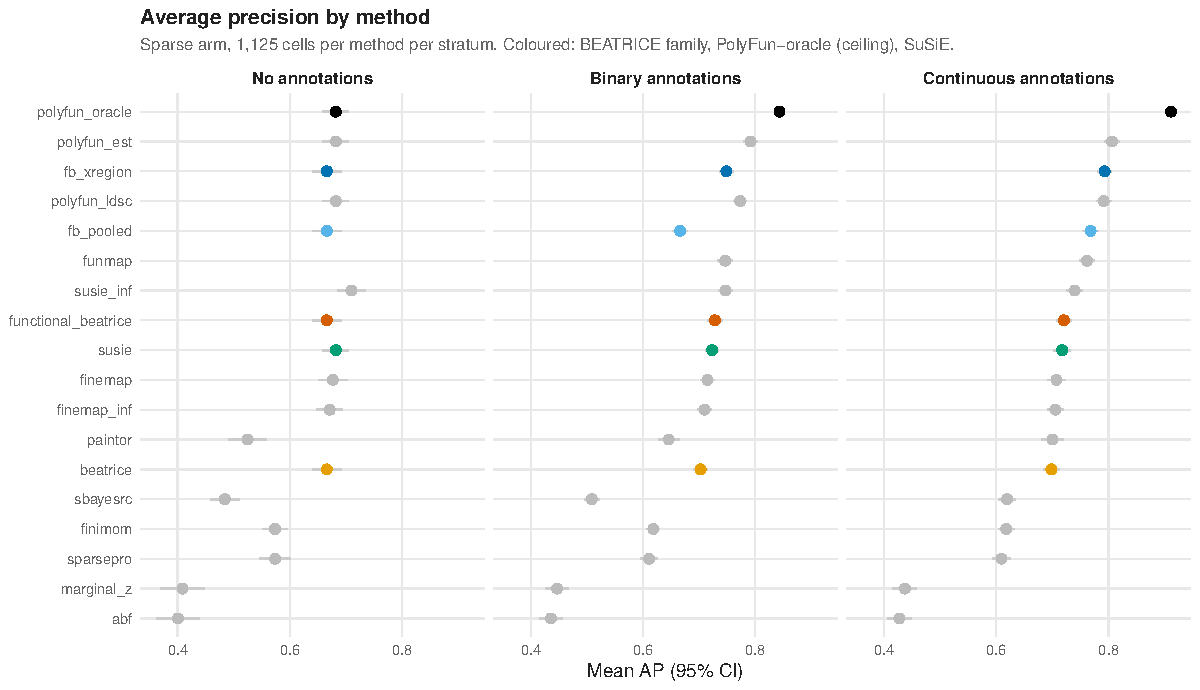
\includegraphics[width=\linewidth]{figs/fig01_ap_ranking.pdf}
\caption{Mean average precision by method, with 95\% intervals over the 1{,}125
cells of each stratum. PolyFun-oracle reads the simulated annotation weights and
is a ceiling, not a deployable competitor.}\label{fig:ap}\end{figure}

Three features of Figure~\ref{fig:ap} are worth stating plainly.

\textbf{The oracle gap is real but not enormous.} PolyFun-oracle sits above
every deployable method on the annotated strata, but the best estimated-prior
methods recover a substantial share of that headroom. On the unannotated arm the
oracle has no information to exploit and collapses onto SuSiE exactly ---
a mechanical check, not a coincidence (\S\ref{sec:validity}).

\textbf{Annotation-aware methods separate from annotation-blind ones only when
annotations exist.} The ordering on the ``none'' panel is essentially a ranking
of sparse-regression quality; the ordering on the annotated panels reorders
substantially.

\textbf{The marginal baselines are informative.} \texttt{marginal\_z} and
\texttt{abf} sit far below everything else, which confirms the design poses a
genuine fine-mapping problem: LD is doing real work, and simply ranking by
marginal significance is not competitive.

\section{When does each method do well?}\label{sec:conditional}

\begin{figure}[htbp]\centering
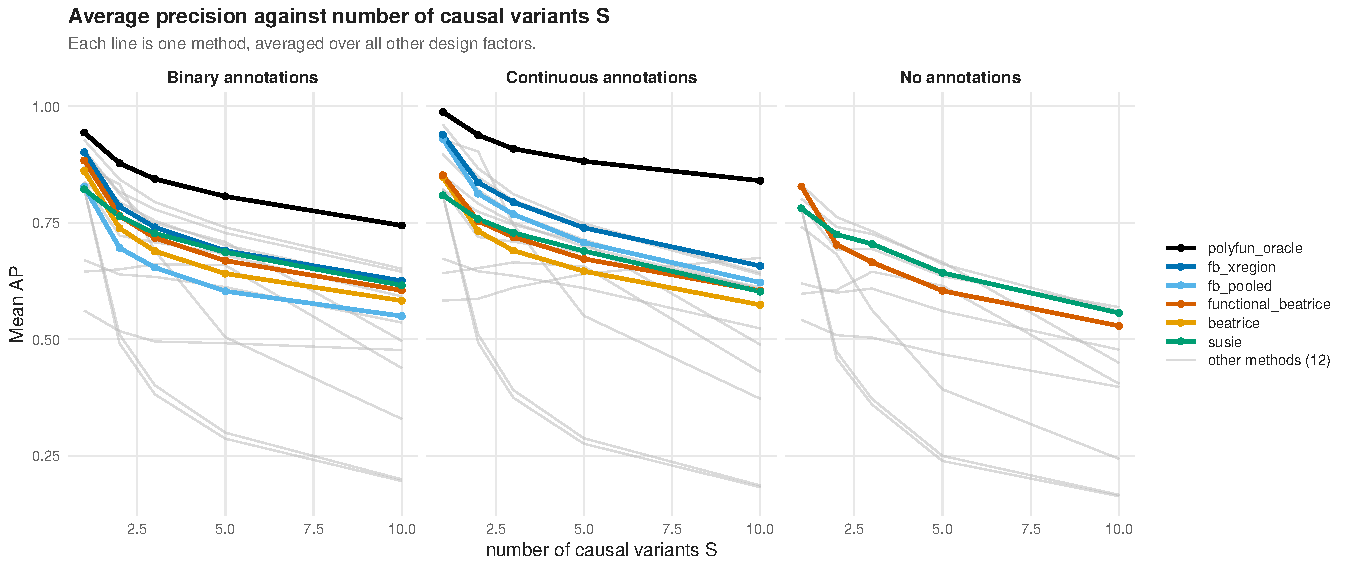
\includegraphics[width=\linewidth]{figs/fig02_ap_vs_S.pdf}
\caption{AP against the number of causal variants. Every method degrades as $S$
grows; the spread between methods also widens.}\label{fig:vs-s}\end{figure}

\begin{figure}[htbp]\centering
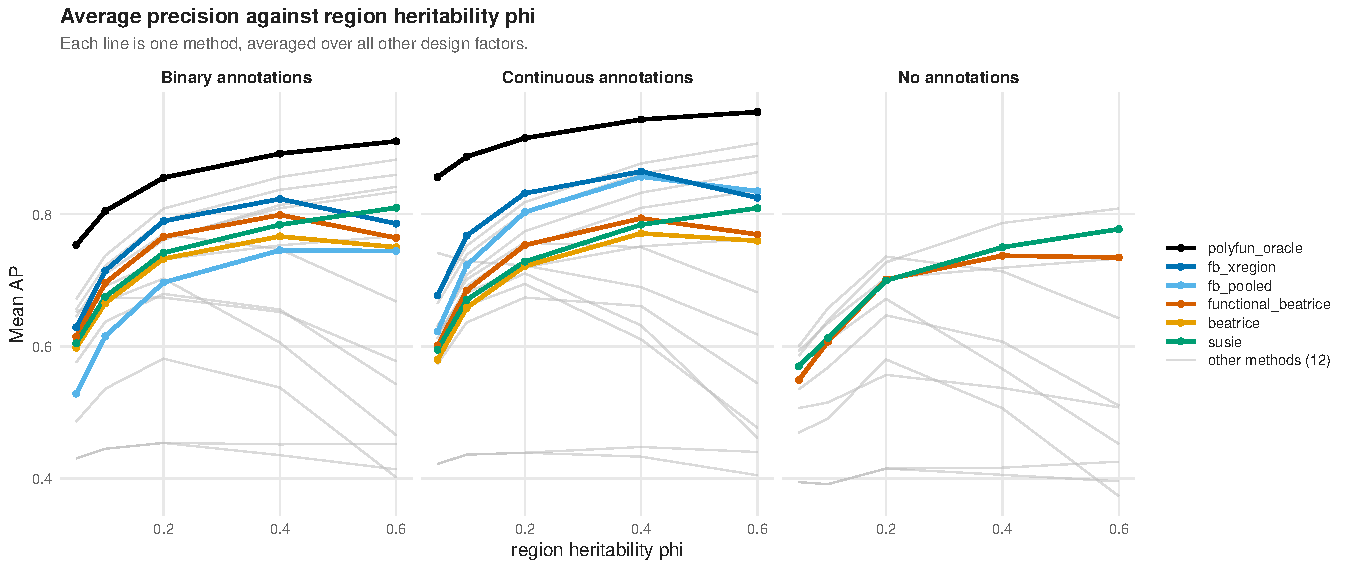
\includegraphics[width=\linewidth]{figs/fig03_ap_vs_phi.pdf}
\caption{AP against region heritability. More signal helps everything, with
diminishing returns at the top of the range.}\label{fig:vs-phi}\end{figure}

\begin{figure}[htbp]\centering
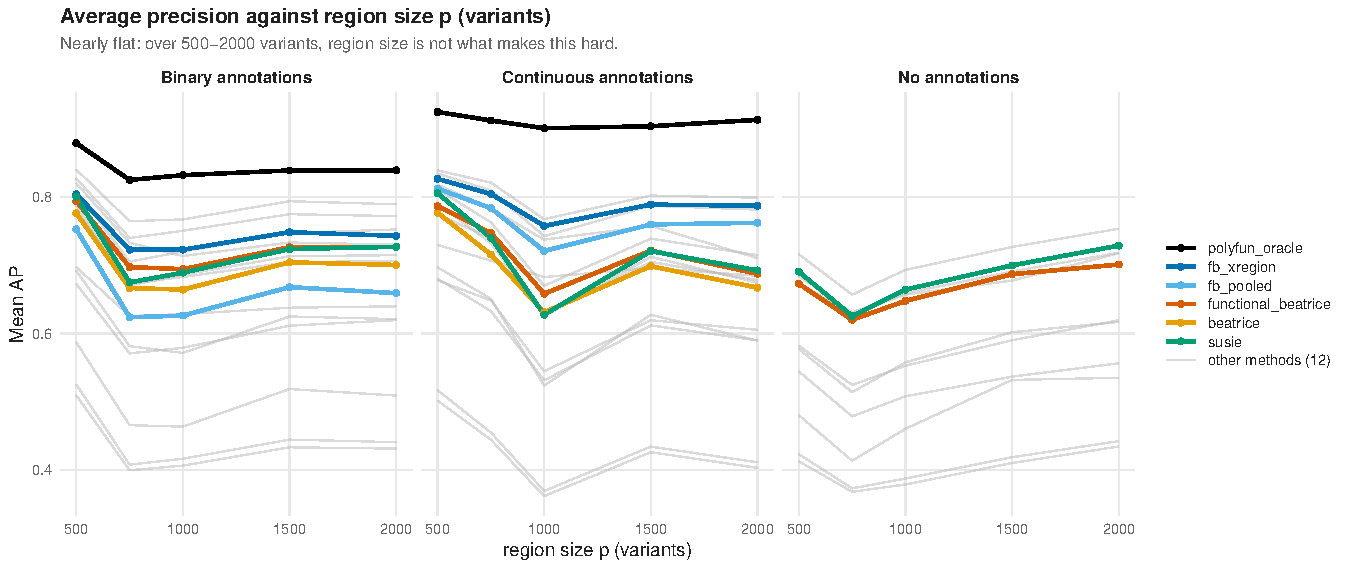
\includegraphics[width=\linewidth]{figs/fig04_ap_vs_p.pdf}
\caption{AP against region size. Nearly flat --- over $500$--$2000$ variants,
region size is not what makes fine-mapping hard here.}\label{fig:vs-p}\end{figure}

\begin{figure}[htbp]\centering
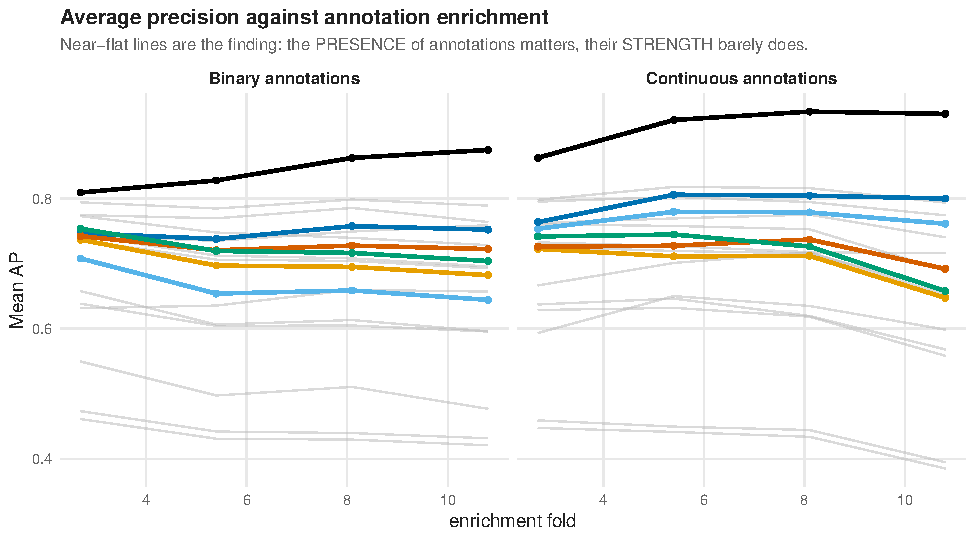
\includegraphics[width=\linewidth]{figs/fig05_ap_vs_enrich.pdf}
\caption{AP against annotation enrichment fold. The near-flat lines are the
result: what matters is that annotations exist, not how strongly they are
enriched over the range swept.}\label{fig:vs-enrich}\end{figure}

The practical summary is that \textbf{sparsity is the binding constraint}.
Moving from $S=1$ to $S=10$ costs far more accuracy than moving from
$\phi=0.6$ to $\phi=0.05$, and both dwarf region size and enrichment strength.
For a practitioner this reframes the question: the useful prior information is
how many independent signals a locus is likely to contain, not how large the
locus is.

\section{False discovery and calibration}\label{sec:calibration}

\begin{figure}[htbp]\centering
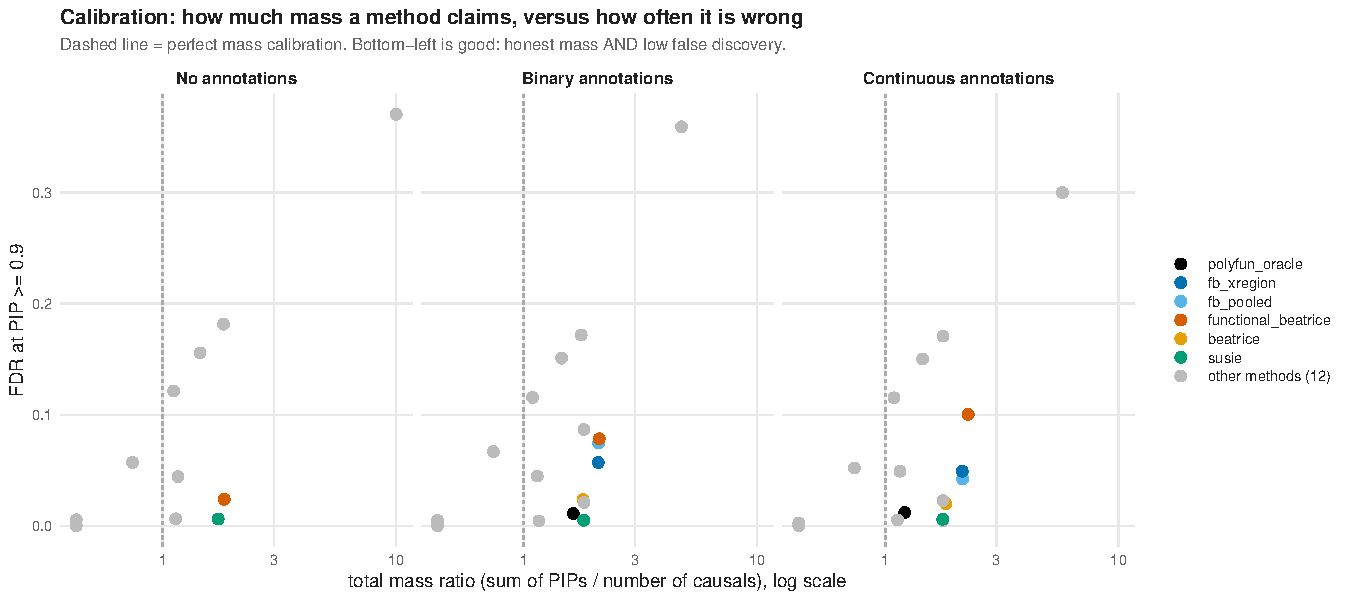
\includegraphics[width=\linewidth]{figs/fig06_calibration_tradeoff.pdf}
\caption{Mass claimed versus errors made. The dashed vertical line is perfect
mass calibration; the bottom-left corner is the desirable
region.}\label{fig:calib}\end{figure}

\begin{figure}[htbp]\centering
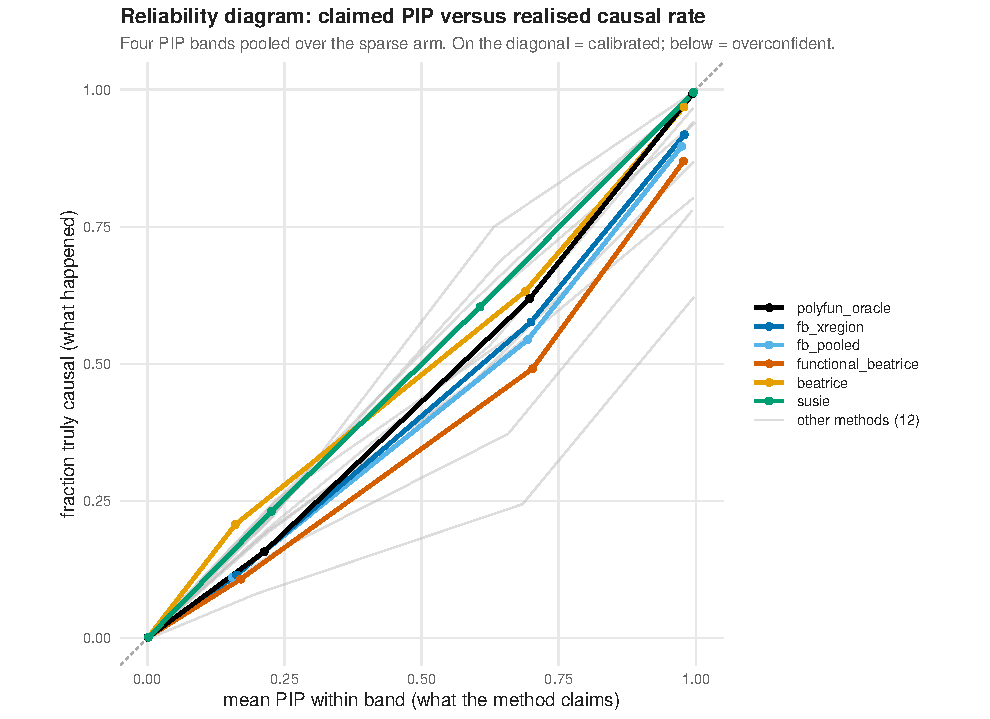
\includegraphics[width=0.78\linewidth]{figs/fig07_reliability.pdf}
\caption{Reliability diagram over the whole sparse arm. Points below the
diagonal are overconfident: the method claimed more probability than the
realised causal rate justified.}\label{fig:reliability}\end{figure}

\begin{figure}[htbp]\centering
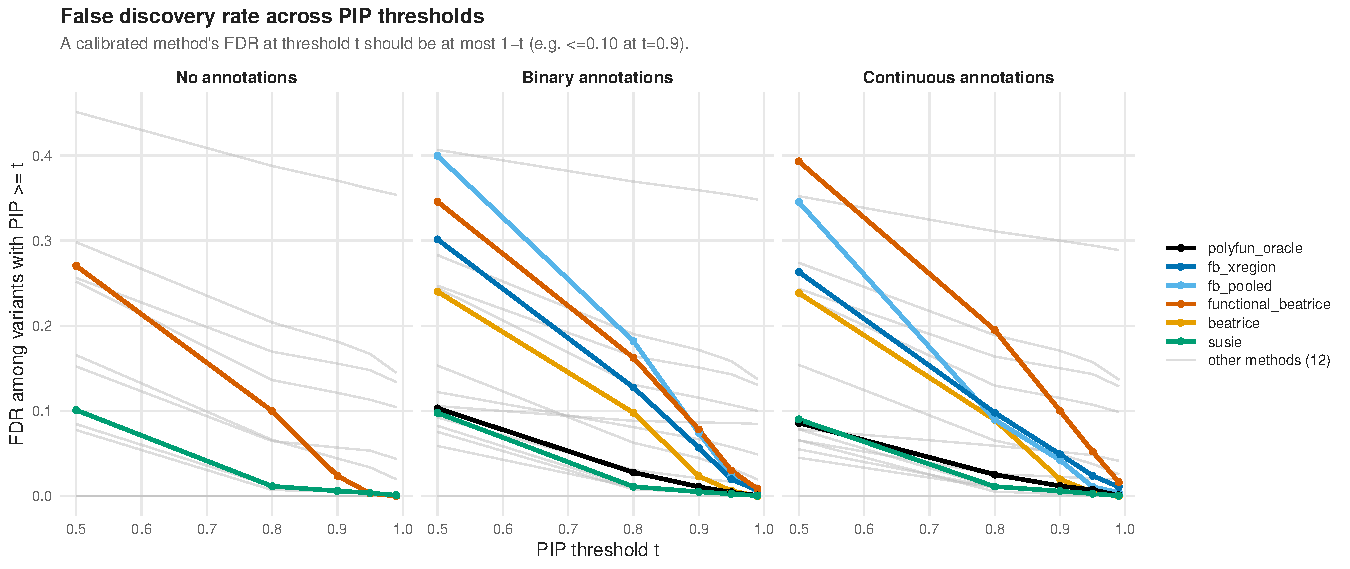
\includegraphics[width=\linewidth]{figs/fig08_fdr_thresholds.pdf}
\caption{FDR as a function of the PIP threshold. A calibrated method should
satisfy $\mathrm{FDR}_t\le 1-t$.}\label{fig:fdr}\end{figure}

\begin{figure}[htbp]\centering
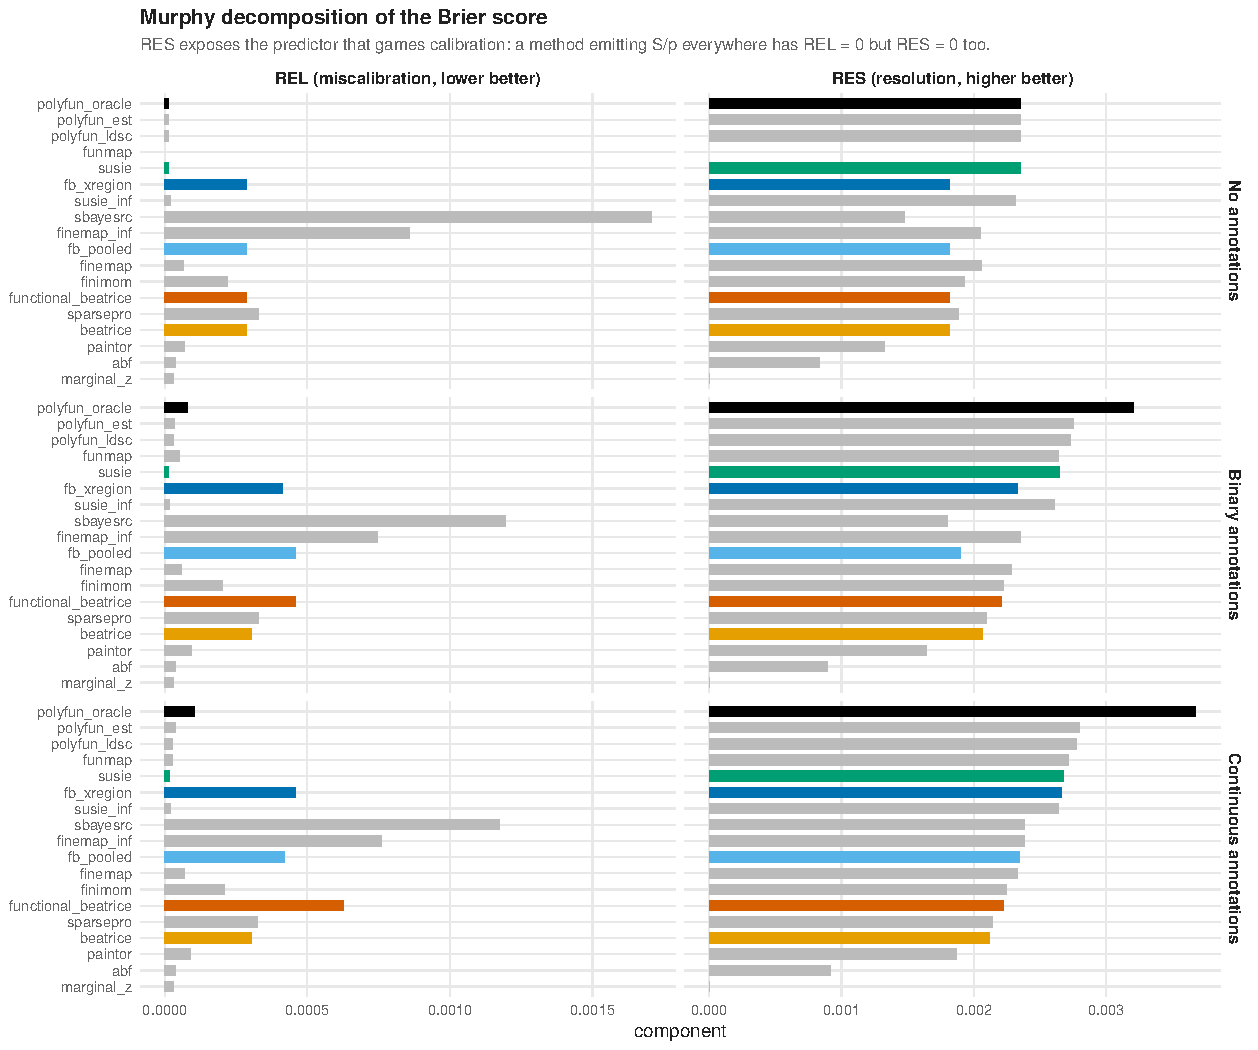
\includegraphics[width=\linewidth]{figs/fig10_murphy.pdf}
\caption{Murphy decomposition. REL is miscalibration (lower is better); RES is
resolution (higher is better). RES is what separates a genuinely informative
posterior from one that is calibrated by being vague.}\label{fig:murphy}\end{figure}

The central trade-off in Figure~\ref{fig:calib} is that \textbf{ranking accuracy
and calibration are not the same axis and the leaders differ}. Methods can be
grouped:

\begin{itemize}
\item \textbf{Conservative and well-calibrated}: SuSiE-inf and FINEMAP hold mass
ratios near $1.1$--$1.2$ with low FDR, at some cost in AP.
\item \textbf{Accurate and mass-inflated}: the BEATRICE family achieves high AP
while claiming roughly twice the mass that exists, with FDR at $\pip\ge0.9$ an
order of magnitude above the PolyFun family.
\item \textbf{Diffuse}: \texttt{sbayesrc} spreads mass extremely widely
(ratios in the multiples), which shows up as both poor calibration and a large
credible-set burden.
\item \textbf{Abstaining}: \texttt{marginal\_z} and \texttt{abf} place very
little mass anywhere; their apparent FDR advantage is a consequence of rarely
crossing the threshold at all, which is exactly why $n_t$ is reported alongside.
\end{itemize}

\section{Credible sets: the follow-up burden}\label{sec:csresults}

\begin{figure}[htbp]\centering
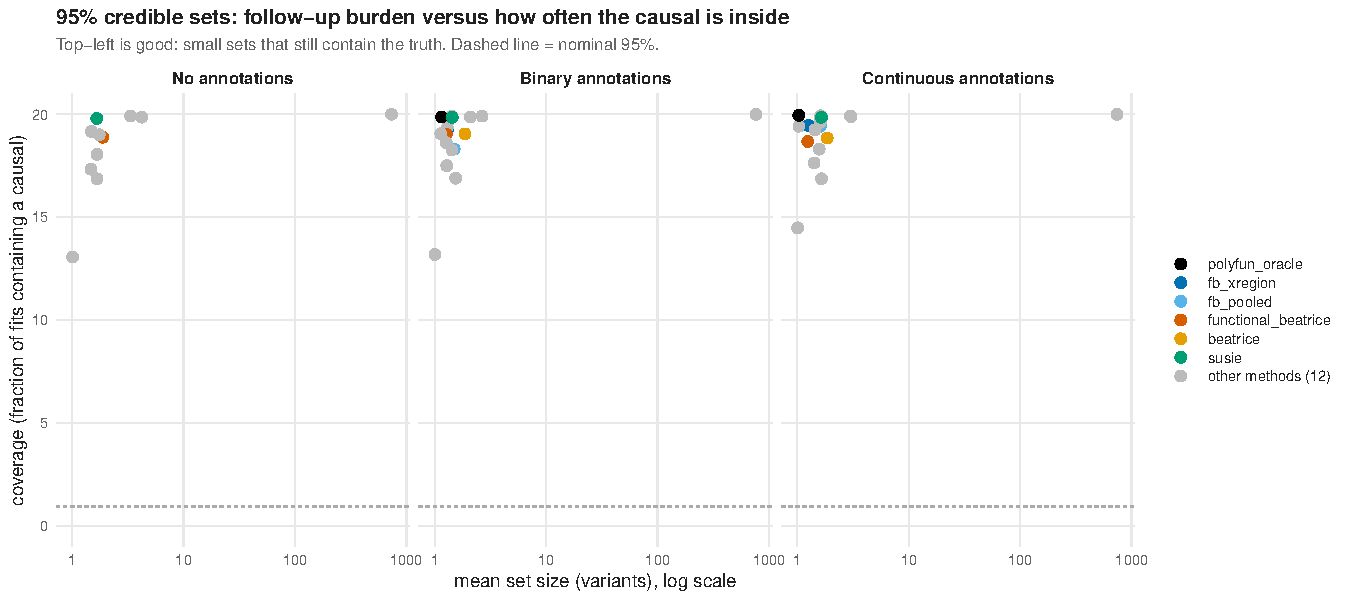
\includegraphics[width=\linewidth]{figs/fig09_credible_sets.pdf}
\caption{95\% credible sets. The practitioner's question is the pair: how many
variants must be taken to the bench, and how often is the causal one among
them.}\label{fig:cs}\end{figure}

Coverage below the nominal $95\%$ combined with small sets indicates a posterior
that is too sharp; coverage at nominal with very large sets indicates one that
is too diffuse. Neither number alone identifies which situation a method is in,
which is why Figure~\ref{fig:cs} plots them jointly and on a log size axis.

\section{Sense V: what moves the metric}\label{sec:sensev}

\begin{figure}[htbp]\centering
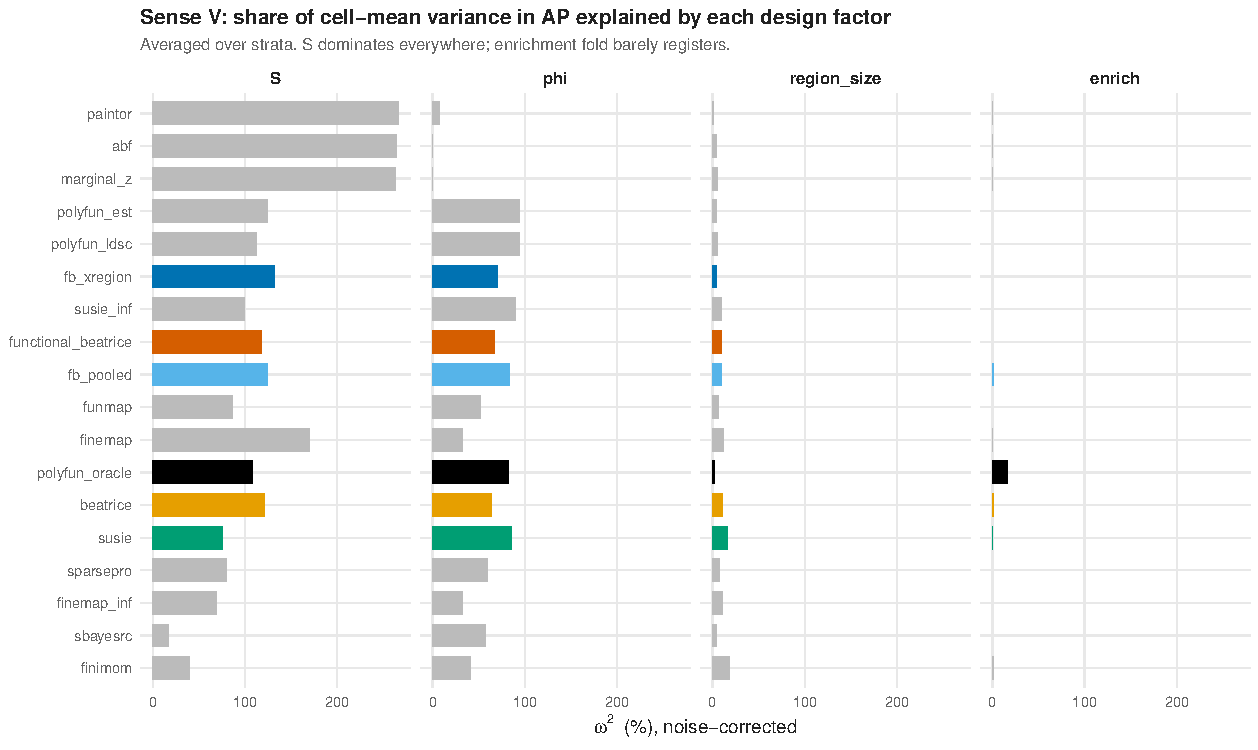
\includegraphics[width=\linewidth]{figs/fig11_sense_v.pdf}
\caption{Noise-corrected $\omega^2$ for each main effect, per method. $S$
dominates; enrichment fold is negligible.}\label{fig:sensev}\end{figure}

Averaged over methods within stratum, the main-effect shares of AP are: $S$
between $38.5\%$ and $46.6\%$; $\phi$ between $19.0\%$ and $21.4\%$; region size
$4.1$--$4.5\%$; enrichment fold $1.2$--$6.1\%$. The largest interaction is
$S{:}\phi$, worth roughly $12$--$14\%$, which is interpretable: heritability per
causal variant, $\phi/S$, is closer to the quantity that actually governs
difficulty than either factor alone.

Because main effects carry the majority of the explained variance, \textbf{the
marginal plots in \S\ref{sec:conditional} are honest summaries} --- claims do not
have to be stated conditionally. Had two-way terms dominated, they would.

\paragraph{A caveat that must travel with these numbers.} $\omega^2$ is defined
relative to the input distribution, here uniform over the levels swept. Widening
a factor's range mechanically inflates its importance. $S$ spans a tenfold range
($1$--$10$) while enrichment spans fourfold ($2.7$--$10.8$), so part of $S$'s
dominance is range. The correct phrasing is always ``$S$ explains $43\%$ of the
variance \emph{over the range swept}'', never ``$S$ is the most important
factor''.

\section{Sense D: what changes the decision}\label{sec:sensed}

\begin{figure}[htbp]\centering
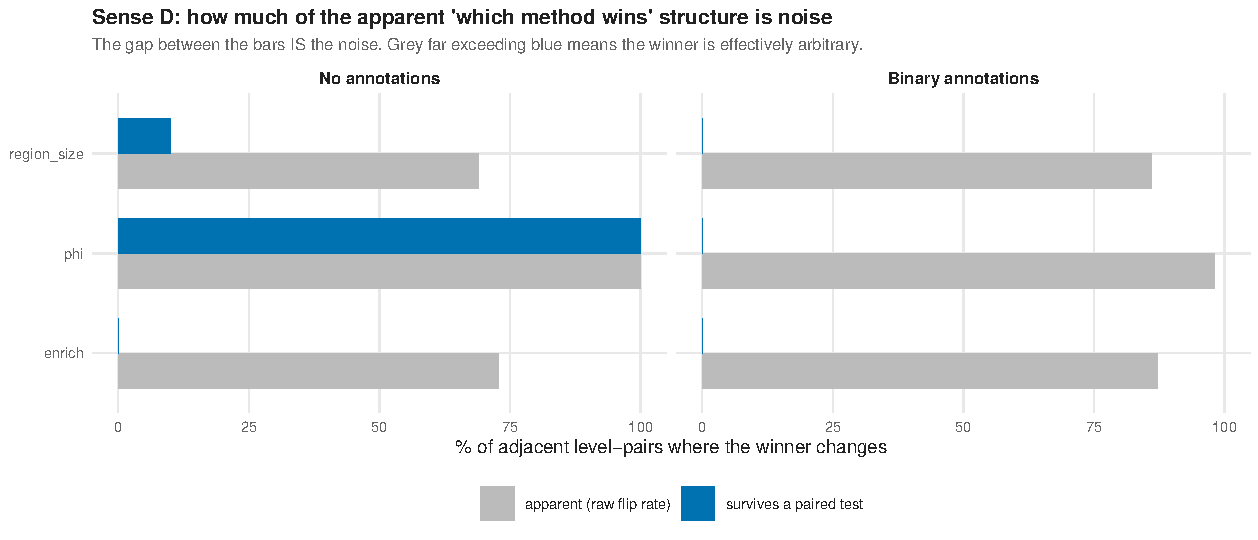
\includegraphics[width=\linewidth]{figs/fig12_sense_d.pdf}
\caption{Apparent versus statistically supported changes of winner. The gap is
the noise.}\label{fig:sensed}\end{figure}

This is the most cautionary result in the report. Raw flip rates are enormous
--- $64\%$ to $100\%$ of adjacent level-pairs show a change in which method
scores best --- while the gated rates collapse to near zero, and only $1.6\%$ to
$7.8\%$ of cells have any statistically decidable winner at all.

\textbf{At 20 fits per cell, the benchmark cannot resolve which of 18 methods is
best within a single cell.} Regime maps built from modal winners are therefore
mostly empty, and the ones that are populated should not be read as
recommendations.

This does \emph{not} contradict \S\ref{sec:senseg}. Those are different
questions with very different power: ``which of 18 methods wins this one cell''
uses 20 fits, whereas ``does method A beat method B on average'' pools thousands
of paired replicates. The benchmark answers the second question decisively and
the first one barely at all --- and reporting both is the honest position.

\section{Sense G: headroom and the Functional BEATRICE ablation}\label{sec:senseg}

\begin{figure}[htbp]\centering
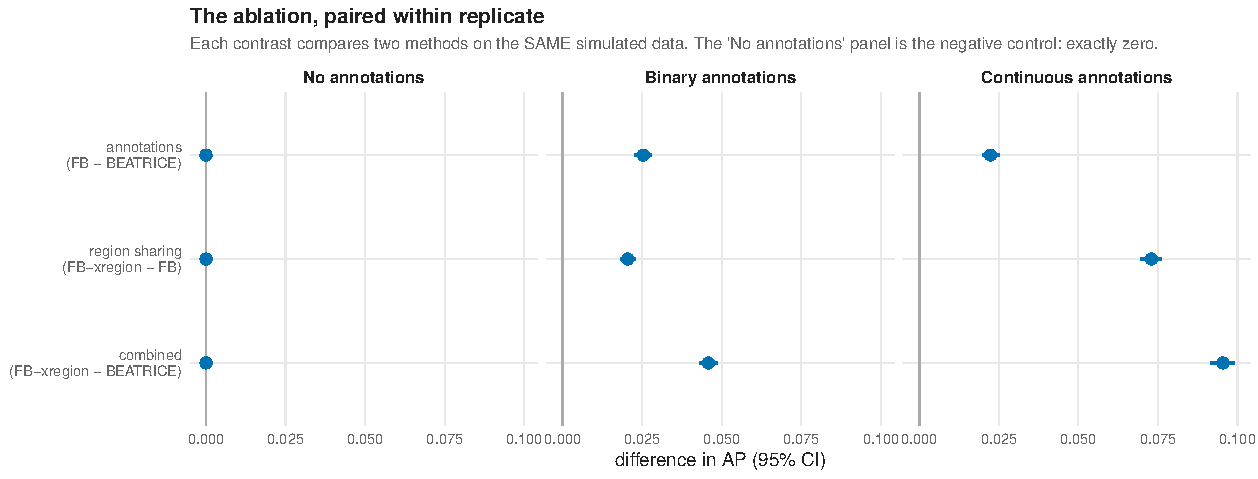
\includegraphics[width=\linewidth]{figs/fig13_ablation.pdf}
\caption{The ablation, paired within replicate. Each contrast compares two
methods on identical simulated data. The ``No annotations'' panel is the
negative control.}\label{fig:ablation}\end{figure}

Because all methods run on the same simulated data, differences can be taken
\emph{within} a replicate, which removes the between-scenario variance that
dominates the marginal comparisons and is what gives this analysis its power.

Table~\ref{tab:ablation} reports the paired contrasts. Both stages of the
ablation are significant, and the negative control is exact:

\begin{itemize}
\item \textbf{Annotations} (Functional BEATRICE $-$ BEATRICE) add
$+0.025$ AP under binary annotations ($t=18.4$) and $+0.022$ under continuous
($t=16.4$).
\item \textbf{Region sharing} (FB-xregion $-$ Functional BEATRICE) adds a
further $+0.021$ ($t=16.8$) and $+0.073$ ($t=43.5$) respectively.
\item \textbf{Combined}, $+0.046$ and $+0.095$ AP.
\item On the unannotated arm all three contrasts are \textbf{exactly
$0.0000\pm0.0000$} over $1{,}250$ paired replicates.
\end{itemize}

That last point deserves emphasis. With no annotations to exploit, the three
variants are bit-identical, so the measured gains cannot be an artefact of the
extra machinery, of additional parameters, or of run-to-run variation. It is as
clean a negative control as the design admits.

Notably, \textbf{region sharing contributes more than annotations alone under
continuous annotations} --- $0.073$ against $0.022$ --- so the extension is not
riding on the base method.

\paragraph{$\kappa$ is reported but should not be over-read.} The headroom
denominator $(\text{ceiling}-\text{baseline})$ is small in many cells, and after
gating out cells with headroom $\le0.02$ the residual $\kappa$ estimates carry
standard deviations of $1.17$--$1.29$ against means between $-0.11$ and $0.31$.
On the unannotated arm the gate removes everything, correctly: with no
annotations the ceiling and the baseline are the same method and $\kappa$ is
undefined by construction. We report $\kappa$ for completeness and rest no
conclusion on it.

\section{Validity checks}\label{sec:validity}

The following are verified mechanically on every run and all pass for the sparse
arm:

\begin{enumerate}
\item In-sample LD only --- zero rows with a reference-panel size.
\item Nine job rows present, matching the grid.
\item Balanced cells per method after documented exclusions --- $1{,}125$ for
every analysed method.
\item No method entirely absent outside the ``none'' arm.
\item \texttt{polyfun\_est} $=$ \texttt{susie} on the unannotated arm.
\item \texttt{polyfun\_ldsc} $=$ \texttt{susie} on the unannotated arm.
\end{enumerate}

Checks 5 and 6 are the strongest structural tests available: both methods reduce
to SuSiE analytically when there are no annotations, so any discrepancy would
indicate a fault in the annotation plumbing rather than in a method. They agree
to numerical precision.

\section{Limitations}\label{sec:limits}

\begin{enumerate}
\item \textbf{In-sample LD only.} Iteration 003 established that in-sample and
reference-panel LD can \emph{invert} method rankings. Nothing here transfers to
the reference-panel setting.
\item \textbf{Sparse architecture only.} This report covers the arm with no
infinitesimal background. The sparse-plus-infinitesimal arm is a separate
analysis.
\item \textbf{Range dependence.} See \S\ref{sec:sensev}; all importance
statements are relative to the ranges swept.
\item \textbf{Per-cell decisions are underpowered.} See \S\ref{sec:sensed}.
\item \textbf{$\kappa$ decomposition unavailable.} The replicate-level table
does not carry the region index, so $\sigma^2_u$ is unidentifiable for the
derived $\kappa$ and $\Delta$ responses. The corrected decomposition is skipped
rather than reported uncorrected, which would inflate whole-plot terms by
$m\sigma^2_u/2$ per degree of freedom.
\item \textbf{One tuning configuration.} BEATRICE-family hyperparameters come
from a single Optuna study and are held fixed; competitors run at their
documented defaults.
\end{enumerate}

\section{Full results tables}\label{sec:tables}

Bold rows are the BEATRICE family. \emph{cells} counts non-missing cells out of
$1{,}125$.

\begin{table}[htbp]\centering\small
\caption{\textbf{No annotations} --- all methods, sparse arm. Ranked by mean AP. \emph{cells} is the number of non-missing cells out of 1{,}125; anything below that is a genuine absence, explained in \S\ref{sec:completeness}.}
\label{tab:main-none}
\begin{tabular}{lrrrrrrrr r}\toprule
method & AP & FDR@.9 & mass & ECE$_{hi}$ & $|CS_{95}|$ & cov$_{95}$ & RES & BSS & cells\\\midrule
susie\_inf & 0.7095 & 0.0062 & 1.14 & 0.0288 & 4.2 & 19.864 & 0.0023 & 0.575 & 125\\
polyfun\_est & 0.6819 & 0.0061 & 1.73 & 0.0225 & 1.7 & 19.800 & 0.0024 & 0.579 & 125\\
polyfun\_ldsc & 0.6819 & 0.0061 & 1.73 & 0.0225 & 1.7 & 19.800 & 0.0024 & 0.579 & 125\\
polyfun\_oracle & 0.6819 & 0.0061 & 1.73 & 0.0225 & 1.7 & 19.800 & 0.0024 & 0.579 & 125\\
susie & 0.6819 & 0.0061 & 1.73 & 0.0225 & 1.7 & 19.800 & 0.0024 & 0.579 & 125\\
finemap & 0.6767 & 0.0442 & 1.16 & 0.0683 & 1.5 & 19.168 & 0.0021 & 0.490 & 125\\
finemap\_inf & 0.6711 & 0.1815 & 1.82 & 0.1619 & 1.7 & 16.864 & 0.0021 & 0.056 & 120\\
\textbf{beatrice} & 0.6659 & 0.0237 & 1.84 & 0.1434 & 1.9 & 18.888 & 0.0018 & 0.321 & 125\\
\textbf{fb\_pooled} & 0.6659 & 0.0237 & 1.84 & 0.1434 & 1.9 & 18.888 & 0.0018 & 0.321 & 125\\
\textbf{fb\_xregion} & 0.6659 & 0.0237 & 1.84 & 0.1434 & 1.9 & 18.888 & 0.0018 & 0.321 & 125\\
\textbf{functional\_beatrice} & 0.6659 & 0.0237 & 1.84 & 0.1434 & 1.9 & 18.888 & 0.0018 & 0.321 & 125\\
sparsepro & 0.5737 & 0.1556 & 1.45 & 0.1232 & 1.5 & 17.336 & 0.0019 & 0.249 & 125\\
finimom & 0.5735 & 0.1213 & 1.12 & 0.0890 & 1.7 & 18.056 & 0.0019 & 0.322 & 125\\
paintor & 0.5247 & 0.0570 & 0.74 & 0.0615 & 1.8 & 19.008 & 0.0013 & 0.372 & 125\\
sbayesrc & 0.4841 & 0.3705 & 10.02 & 0.2207 & 1.0 & 13.064 & 0.0015 & -0.552 & 125\\
marginal\_z & 0.4086 & 0.0000 & 0.43 & NaN & 735.6 & 20.000 & 0.0000 & -0.003 & 125\\
abf & 0.4005 & 0.0054 & 0.43 & 0.0237 & 3.3 & 19.920 & 0.0008 & 0.314 & 125\\
funmap & NaN & 0.0000 & NaN & NaN & NaN & 0.000 & NaN & NaN & 0\\
\bottomrule\end{tabular}\end{table}
\begin{table}[htbp]\centering\small
\caption{\textbf{Binary annotations} --- all methods, sparse arm. Ranked by mean AP. \emph{cells} is the number of non-missing cells out of 1{,}125; anything below that is a genuine absence, explained in \S\ref{sec:completeness}.}
\label{tab:main-binary}
\begin{tabular}{lrrrrrrrr r}\toprule
method & AP & FDR@.9 & mass & ECE$_{hi}$ & $|CS_{95}|$ & cov$_{95}$ & RES & BSS & cells\\\midrule
polyfun\_oracle & 0.8432 & 0.0110 & 1.63 & 0.0715 & 1.2 & 19.866 & 0.0032 & 0.694 & 500\\
polyfun\_est & 0.7914 & 0.0046 & 1.81 & 0.0376 & 1.4 & 19.914 & 0.0028 & 0.644 & 500\\
polyfun\_ldsc & 0.7732 & 0.0209 & 1.81 & 0.0440 & 1.3 & 19.668 & 0.0027 & 0.635 & 500\\
\textbf{fb\_xregion} & 0.7484 & 0.0569 & 2.08 & 0.1454 & 1.3 & 19.306 & 0.0023 & 0.301 & 500\\
susie\_inf & 0.7470 & 0.0043 & 1.16 & 0.0283 & 2.1 & 19.870 & 0.0026 & 0.620 & 500\\
funmap & 0.7462 & 0.0866 & 1.81 & 0.0746 & 1.3 & 18.616 & 0.0026 & 0.614 & 500\\
\textbf{functional\_beatrice} & 0.7280 & 0.0783 & 2.10 & 0.1547 & 1.3 & 19.034 & 0.0022 & 0.245 & 500\\
susie & 0.7232 & 0.0050 & 1.80 & 0.0218 & 1.4 & 19.856 & 0.0026 & 0.624 & 500\\
finemap & 0.7147 & 0.0447 & 1.14 & 0.0648 & 1.3 & 19.346 & 0.0023 & 0.535 & 500\\
finemap\_inf & 0.7096 & 0.1717 & 1.76 & 0.1585 & 1.5 & 16.894 & 0.0024 & 0.141 & 480\\
\textbf{beatrice} & 0.7026 & 0.0235 & 1.79 & 0.1592 & 1.9 & 19.050 & 0.0021 & 0.369 & 500\\
\textbf{fb\_pooled} & 0.6661 & 0.0745 & 2.09 & 0.1547 & 1.5 & 18.312 & 0.0019 & 0.187 & 500\\
paintor & 0.6458 & 0.0668 & 0.74 & 0.0919 & 1.1 & 19.064 & 0.0016 & 0.452 & 500\\
finimom & 0.6182 & 0.1156 & 1.09 & 0.0876 & 1.4 & 18.264 & 0.0022 & 0.378 & 500\\
sparsepro & 0.6107 & 0.1509 & 1.45 & 0.1232 & 1.3 & 17.504 & 0.0021 & 0.286 & 500\\
sbayesrc & 0.5086 & 0.3592 & 4.74 & 0.2470 & 1.0 & 13.186 & 0.0018 & -0.313 & 500\\
marginal\_z & 0.4467 & 0.0000 & 0.43 & NaN & 765.5 & 20.000 & 0.0000 & -0.003 & 500\\
abf & 0.4357 & 0.0047 & 0.43 & 0.0255 & 2.7 & 19.914 & 0.0009 & 0.334 & 500\\
\bottomrule\end{tabular}\end{table}
\begin{table}[htbp]\centering\small
\caption{\textbf{Continuous annotations} --- all methods, sparse arm. Ranked by mean AP. \emph{cells} is the number of non-missing cells out of 1{,}125; anything below that is a genuine absence, explained in \S\ref{sec:completeness}.}
\label{tab:main-continuous}
\begin{tabular}{lrrrrrrrr r}\toprule
method & AP & FDR@.9 & mass & ECE$_{hi}$ & $|CS_{95}|$ & cov$_{95}$ & RES & BSS & cells\\\midrule
polyfun\_oracle & 0.9114 & 0.0119 & 1.21 & 0.0791 & 1.0 & 19.952 & 0.0037 & 0.774 & 500\\
polyfun\_est & 0.8061 & 0.0051 & 1.77 & 0.0414 & 1.6 & 19.928 & 0.0028 & 0.641 & 500\\
\textbf{fb\_xregion} & 0.7933 & 0.0491 & 2.14 & 0.1529 & 1.3 & 19.462 & 0.0027 & 0.327 & 500\\
polyfun\_ldsc & 0.7914 & 0.0047 & 1.77 & 0.0360 & 1.6 & 19.906 & 0.0028 & 0.638 & 500\\
\textbf{fb\_pooled} & 0.7681 & 0.0422 & 2.15 & 0.1504 & 1.6 & 19.424 & 0.0023 & 0.278 & 500\\
funmap & 0.7617 & 0.0227 & 1.77 & 0.0367 & 1.6 & 19.610 & 0.0027 & 0.628 & 500\\
susie\_inf & 0.7398 & 0.0053 & 1.13 & 0.0284 & 3.0 & 19.886 & 0.0026 & 0.618 & 500\\
\textbf{functional\_beatrice} & 0.7204 & 0.1002 & 2.27 & 0.1728 & 1.2 & 18.680 & 0.0022 & 0.117 & 500\\
susie & 0.7175 & 0.0059 & 1.77 & 0.0236 & 1.6 & 19.852 & 0.0027 & 0.621 & 500\\
finemap & 0.7071 & 0.0492 & 1.16 & 0.0682 & 1.4 & 19.250 & 0.0023 & 0.529 & 500\\
finemap\_inf & 0.7053 & 0.1708 & 1.77 & 0.1555 & 1.6 & 16.870 & 0.0024 & 0.143 & 480\\
paintor & 0.7001 & 0.0520 & 0.74 & 0.0790 & 1.0 & 19.420 & 0.0019 & 0.520 & 500\\
\textbf{beatrice} & 0.6981 & 0.0198 & 1.82 & 0.1531 & 1.9 & 18.846 & 0.0021 & 0.362 & 500\\
sbayesrc & 0.6192 & 0.3000 & 5.75 & 0.1993 & 1.0 & 14.482 & 0.0024 & -0.254 & 500\\
finimom & 0.6177 & 0.1152 & 1.09 & 0.0910 & 1.6 & 18.308 & 0.0022 & 0.378 & 500\\
sparsepro & 0.6093 & 0.1502 & 1.45 & 0.1236 & 1.4 & 17.636 & 0.0021 & 0.294 & 500\\
marginal\_z & 0.4371 & 0.0000 & 0.43 & NaN & 738.4 & 20.000 & 0.0000 & -0.003 & 500\\
abf & 0.4271 & 0.0024 & 0.43 & 0.0237 & 3.0 & 19.910 & 0.0009 & 0.333 & 500\\
\bottomrule\end{tabular}\end{table}
\begin{table}[htbp]\centering\small
\caption{Paired ablation on AP. Each row compares two methods on the \emph{same} simulated replicate; $n$ is the number of paired replicates. $t=\bar d/\mathrm{SE}(\bar d)$.}\label{tab:ablation}
\begin{tabular}{llrrrrr}\toprule
stratum & contrast & $\bar d$ & sd & $n$ & SE & $t$\\\midrule
No annotations & annotations & 0.0000 & 0.0000 & 1250 & 0.00000 & ---\\
No annotations & region sharing & 0.0000 & 0.0000 & 1250 & 0.00000 & ---\\
No annotations & combined & 0.0000 & 0.0000 & 1250 & 0.00000 & ---\\
Binary annotations & annotations & 0.0254 & 0.0975 & 4981 & 0.00138 & 18.4\\
Binary annotations & region sharing & 0.0205 & 0.0859 & 4980 & 0.00122 & 16.8\\
Binary annotations & combined & 0.0458 & 0.1026 & 4980 & 0.00145 & 31.5\\
Continuous annotations & annotations & 0.0224 & 0.0962 & 4965 & 0.00136 & 16.4\\
Continuous annotations & region sharing & 0.0730 & 0.1183 & 4960 & 0.00168 & 43.5\\
Continuous annotations & combined & 0.0954 & 0.1352 & 4960 & 0.00192 & 49.7\\
\bottomrule\end{tabular}\end{table}


\end{document}
